
%%%%%%%%%%%%%%%%%%%%%%% file typeinst.tex %%%%%%%%%%%%%%%%%%%%%%%%%
%
% This is the LaTeX source for the instructions to authors using
% the LaTeX document class 'llncs.cls' for contributions to
% the Lecture Notes in Computer Sciences series.
% http://www.springer.com/lncs       Springer Heidelberg 2006/05/04
%
% It may be used as a template for your own input - copy it
% to a new file with a new name and use it as the basis
% for your article.
%
% NB: the document class 'llncs' has its own and detailed documentation, see
% ftp://ftp.springer.de/data/pubftp/pub/tex/latex/llncs/latex2e/llncsdoc.pdf
%
%%%%%%%%%%%%%%%%%%%%%%%%%%%%%%%%%%%%%%%%%%%%%%%%%%%%%%%%%%%%%%%%%%%


\documentclass[runningheads,a4paper]{llncs}

\usepackage{amssymb}
\setcounter{tocdepth}{3}
\usepackage{graphicx}
\usepackage{epstopdf}

\usepackage{url}
\urldef{\mailsa}\path|{up201305378, up201303501} @fe.up.pt |    
\urldef{\mailsb}\path| FEUP-PLOG, Turma 3MIEIC06, Grupo Akkoy_2 |
\newcommand{\keywords}[1]{\par\addvspace\baselineskip
\noindent\keywordname\enspace\ignorespaces#1}

\begin{document}

\mainmatter  % start of an individual contribution

% first the title is needed
\title{The use of restrictions in Logic Programming:\\Puzzle Akkoy}

% a short form should be given in case it is too long for the running head
\titlerunning{The use of restrictions in Logic Programming: Puzzle Akkoy}

% the name(s) of the author(s) follow(s) next
%
% NB: Chinese authors should write their first names(s) in front of
% their surnames. This ensures that the names appear correctly in
% the running heads and the author index.
%
\author{Filipa Ramos
\and Ines Santos}
%
\authorrunning{The use of restrictions in Logic Programming: Puzzle Akkoy}
% (feature abused for this document to repeat the title also on left hand pages)

% the affiliations are given next; don't give your e-mail address
% unless you accept that it will be published
\institute{Faculdade de Engenharia da Universidade do Porto,\\
Rua Dr. Roberto Frias, 4200 - 465, Porto, Portugal\\
\mailsa\\
\mailsb\\
\url{https://sigarra.up.pt/feup/pt/web_page.inicial}}

%
% NB: a more complex sample for affiliations and the mapping to the
% corresponding authors can be found in the file "llncs.dem"
% (search for the string "\mainmatter" where a contribution starts).
% "llncs.dem" accompanies the document class "llncs.cls".
%

\toctitle{The use of restrictions in Logic Programming}
\tocauthor{Puzzle Akkoy}
\maketitle


\begin{abstract}
The present report serves the purpose of explaning the process of finding a solution for akkoy puzzles using programming with restrictions. It also refers the implementation of restrictions in order to generate random puzzles. The main objective is to deepen the knowledge of \emph {PROLOG}, specially the clpfd library. The project was developed for the curricular unit of Logic Programming. The results will be evaluated in order to realize the efficiency of the found solution.
\keywords{restrictions programming logic prolog efficiency}
\end{abstract}


\section{Introduction}

This project was developed for the curricular unit of Logic Programming in order to deepen the knowledge of the clpfd prolog library. Between the many objectives accounted for this project, the following can be highlighted: examining the results of the use of restrictions whilst programming, understanding the logic of rule-based languages, realizing the advantages of logic in programming. The analized puzzle has many restrictions which made it hard to find a solution which incorporated all the restrictions. Besides this, the efficiency of the solution can not be hightened as well as in other puzzles since the difficulty level is very high. The implemented solution uses the following approach: count the number of black squares in columns and white squares in lines and compare it with the numbers on the restrictions list. The returned board is a list of variables. Each number one represents a black square and each number two represents a white square. 
The article is structured in order to make it easier to understand the solution. Firstly, the problem is described. Secondly, the solution and its visualization is explained. Finally, the results are analized and the conclusions are made. 

\section {Problem Description}



\section {Approach}



\subsection{Decision Variables}

\subsection{Constraints}

\subsection{Search Strategy}



\section{Solution Presentation}


\section{Results}

The numbers accorded to lemmas, propositions, and theorems, etc. should
appear in consecutive order, starting with Lemma 1, and not, for
example, with Lemma 11.

\section{Conclusions and Future Work}

\begin{figure}
\centering
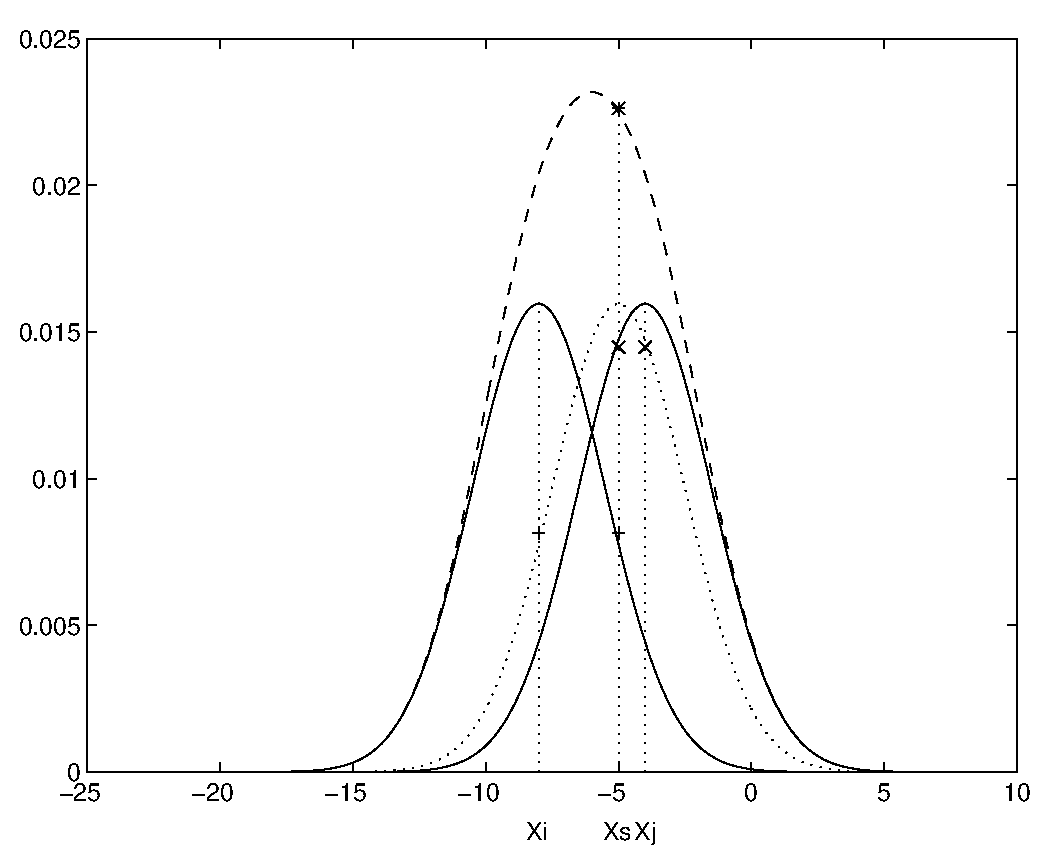
\includegraphics[height=6.2cm]{eijkel2}
\caption{One kernel at $x_s$ (\emph{dotted kernel}) or two kernels at
$x_i$ and $x_j$ (\textit{left and right}) lead to the same summed estimate
at $x_s$. This shows a figure consisting of different types of
lines. Elements of the figure described in the caption should be set in
italics, in parentheses, as shown in this sample caption.}
\label{fig:example}
\end{figure}


\section{References}

\begin{thebibliography}{4}

\bibitem{jour} Smith, T.F., Waterman, M.S.: Identification of Common Molecular
Subsequences. J. Mol. Biol. 147, 195--197 (1981)

\bibitem{lncschap} May, P., Ehrlich, H.C., Steinke, T.: ZIB Structure Prediction Pipeline:
Composing a Complex Biological Workflow through Web Services. In: Nagel,
W.E., Walter, W.V., Lehner, W. (eds.) Euro-Par 2006. LNCS, vol. 4128,
pp. 1148--1158. Springer, Heidelberg (2006)

\bibitem{book} Foster, I., Kesselman, C.: The Grid: Blueprint for a New Computing
Infrastructure. Morgan Kaufmann, San Francisco (1999)

\bibitem{proceeding1} Czajkowski, K., Fitzgerald, S., Foster, I., Kesselman, C.: Grid
Information Services for Distributed Resource Sharing. In: 10th IEEE
International Symposium on High Performance Distributed Computing, pp.
181--184. IEEE Press, New York (2001)

\bibitem{proceeding2} Foster, I., Kesselman, C., Nick, J., Tuecke, S.: The Physiology of the
Grid: an Open Grid Services Architecture for Distributed Systems
Integration. Technical report, Global Grid Forum (2002)

\bibitem{url} National Center for Biotechnology Information, \url{http://www.ncbi.nlm.nih.gov}

\end{thebibliography}


\section{Annex}

\begin{equation}
  \psi (u) = \int_{o}^{T} \left[\frac{1}{2}
  \left(\Lambda_{o}^{-1} u,u\right) + N^{\ast} (-u)\right] dt \;  .
\end{equation}


\end{document}
